\documentclass[12 pt]{article}
\usepackage{hyperref}
\usepackage{fancyhdr}
\usepackage{setspace}
\usepackage{enumerate}
\usepackage{amsmath}
\usepackage{lastpage}
\usepackage{mathtools,float}
\usepackage{tikz}
\usepackage[margin=1 in]{geometry}
\usepackage{amsthm}
\newtheorem{thm}{Theorem}
\theoremstyle{definition}
\newtheorem{defn}{Definition}
%\newtheorem{def}{Definition}
\usepackage{amssymb}
\usepackage{gensymb}
\allowdisplaybreaks
%\usepackage[dvipsnames]{xcolor}   %May be necessary if you want to color links
\hypersetup{
	%colorlinks=true, %set true if you want colored links
	linktoc=all,     %set to all if you want both sections and subsections linked
	linkcolor=black,  %choose some color if you want links to stand out
}
\usepackage{graphicx}
\graphicspath{{Images/}}
\author{Julian Lore}
\date{Last updated: \today}
\title{MATH 222: Calculus III Review}
\pagestyle{fancy}
\lhead{MATH 222}
\chead{\leftmark}
\rhead{Julian Lore}
\cfoot{Page \thepage \ of \pageref{LastPage}}
\newcommand{\tab}[1]{\hspace{.2\textwidth}\rlap{#1}}
\begin{document}
	\onehalfspacing
	\maketitle
	Adapted from Alexander Garver's Winter 2017 MATH222 lecture notes.
	\tableofcontents
	\newpage
	%\section{Sequences}
	%List of real numbers, convergent if it has a limit. Increasing sequence has a limit when it has an upper bound.
	\section{Series}
	$n^{th}$ partial sum of a sequence. $a_n$, the terms of the series, must tend to $0$, or else the series \textbf{diverges}.
	\subsection{Special Series}
	\paragraph{Harmonic} $\sum_{n=1}^{\infty} \frac{1}{n}$ diverges.
	\paragraph{Geometric} $\sum_{n=1}^{\infty}r^n$ converges to $\frac{1}{1-r}$ $\iff$ $-1<r<1$.
	\subsection{Tests}
	\paragraph{Alternating Series Test/Leibniz Test}
	Sequence $a_1,a_2,\ldots$ is \textbf{decreasing} and has limit $0$. Then $\sum_{n=1}^{\infty}(-1)^n a_n$ converges. In other words, absolute value of the alternating series forms a convergence sequence.
	\paragraph{Absolute Convergence Test}
	$\sum_{n=1}^{\infty}|a_n|$ converges $\implies \sum_{n=1}^{\infty}a_n$ converges.
	\paragraph{Ratio Test} Suppose $\lim_{n\to \infty} \left|\frac{a_{n+1}}{a_n}\right|=r$. 
	\\$r<1 \implies \sum_{n=1}^{\infty}|a_n|$ converges and 
	\\$r>1 \implies \sum_{n=1}^{\infty}a_n$ diverges.
	\paragraph{Root Test} Suppose $\lim_{n\to \infty}\sqrt[n]{|a_n|}=r$. 
	\\$r<1 \implies \sum_{n=1}^{\infty}|a_n|$ converges and 
	\\$r>1 \implies \sum_{n=1}^{\infty}a_n$ diverges.
	\paragraph{Comparison Test} Suppose fixed number $K$ s.t. $0<a_n<Kb_n$, $\forall$ sufficiently large $n$. 
	\\ $\sum_{n=1}^{\infty}b_n$ converges $\implies \sum_{n=1}^{\infty} a_n$ converges.
	\\ $\sum_{n=1}^{\infty}a_n$ diverges $\implies \sum_{n=1}^{\infty} b_n$ diverges.
	\paragraph{Limit Comparison Test} Suppose $a_n>0,b_n>0$ and $\lim_{n\to \infty}\frac{a_n}{b_n}=R\neq 0$. Then $\sum_{n=1}^{\infty}a_n$ and $\sum_{n=1}^{\infty}b_n$ \textbf{both} converge or \textbf{both} diverge.
	\paragraph{Integral Test} Suppose $f(x)$ is \textbf{positive} and \textbf{decreasing}, $\forall$ large enough $x$. Then the following are equivalent:
	\begin{enumerate}[1)]
		\item $\int_{1}^{\infty} f(x)dx$ is finite, i.e. converges.
		\item $\sum_{n=1}^{\infty}f(n)$ is finite, i.e. converges.
	\end{enumerate}
The p-test follows from this.
\subparagraph{$p$-test}
$\sum_{n=1}^{\infty} \frac{1}{n^p}$ converges $\iff$ $p>1$.
\paragraph{Alternating Series Estimation Theorem} If $s=\sum_{n=1}^{\infty}(-1)^{n-1}b_n$ is the sum of an alternating series that satisfies:
\\ $b_{n+1}\leq b_n$ and $\lim_{n\to \infty}b_n=0$
\\ then $|R_n|=|s-s_n|\leq b_{n+1}$.
\subsection{Power Series}Series of the form $\sum_{n=0}^{\infty}c_n x^n$ or $\sum_{n=0}^{\infty}c_n(x-a)^n$

\subsubsection{Important Power Series to Know}
\begin{itemize}
	\item $e^x=\sum_{n=0}^{\infty}\frac{x^n}{n!}, R=\infty$
	\item $\sin{x}=\sum_{n=0}^{\infty}(-1)^n \frac{x^{2n+1}}{(2n+1)!},R=\infty$
	\item $\cos{x}=\sum_{n=0}^{\infty}(-1)^n \frac{x^{2n}}{(2n)!}, R=\infty$
	\item $\tan^{-1}{x}=\sum_{n=0}^{\infty}(-1)^n \frac{x^{2n+1}}{2n+1}, R=1$
	\item $\ln{(1+x)}=\sum_{n=1}^{\infty}(-1)^{n-1}\frac{x^n}{n}, R=1$
\end{itemize}
\subsubsection{Convergence}
\begin{thm}
	$\sum_{n=0}^{\infty}c_n(x-a)^n$ does exactly one of the following:
	\begin{enumerate}[(i)]
		\item Converges only when $x=a$.
		\item Converges for all $x$.
		\item $\exists$ $R>0$ s.t. $|x-a|<R$, the series converges and diverges if $|x-a|>R$.
	\end{enumerate}
\end{thm}
	R is the \textbf{radius of convergence}. The values of $x$ where the series converges is called the \textbf{interval of convergence}. Radius of convergence \textbf{does not} tell you if endpoints are included, have to check both. Ratio test is usually a good tool to find the radius of convergence.
	\subsubsection{Representing Functions As Power Series}
	If $f(x)=\sum_{n=0}^{\infty}c_n(x-a)^n$ for some $c_0,c_1,\ldots$ then $f'(x)$ and $\int f(x) dx$ can also be represented by a power series.
	\\ If $f(x)=\sum_{n=0}^{\infty}c_n(x-a)$ then $c_n=\frac{f^{n}(a)}{n!}$
	\\ Work with a familiar power series: $\sum_{n=0}^{\infty}x^n=\frac{1}{1-x}$ for $|x|<1$.
	\begin{thm}
		Suppose $\sum_{n=0}^{\infty}c_n(x-a)^n$ with $R>0$. Then $f(x)=\sum_{n=0}^{\infty}c_n(x-a)^n$ is differentiable on $(a-R,a+R)$ and 
		\begin{enumerate}[1)]
			\item $f'(x)=c_1+2c_2(x-a)+3c_3(x-a)^2+\ldots$
			\item $\int f(x) dx=c+c_0(x-a)+\frac{c_1}{2}(x-a)^2+\frac{c_2}{3}(x-a)^3+\ldots$
		\end{enumerate}
	The radius of convergence of $f'(x)$ and $\int f(x)dx$ is $R$.
	\end{thm} Otherwise said, you can easily differentiate \& integrate series.
	\begin{thm}
		If $f(x)$ has a power series representation $\sum_{n=0}^{\infty} c_n (x-a)^n$ then $c_n=\frac{f^{n}(a)}{n!}$. Called the $n!$ \textbf{Taylor series} of $f$ at $a$.
	\end{thm}
	How to show a function is represented by a power series?
	\begin{thm}
		Suppose $\sum_{n=0}^{\infty} c_n(x-a)^n$ is the Taylor series of $f(x)$ with $R>0$. \\If $\lim_{n\to \infty} (f(x)-\sum_{i=0}^{\infty}c_i(x-a)^i)=0$ for $|x-a|<R$, then $f(x)=\sum_{n=0}^{\infty}c_n(x-a)^n$ for $|x-a|<R$.
	\end{thm}
	\section{3-Dimensional Coordinate System}
	$XYZ$ plane. 
	\paragraph{Distance Between 2 Points, $P$ and $Q$}
	$$|PQ|=\sqrt{(a_2-a_1)^2+(b_2-b_1)^2+(c_2-c_1)^2}$$
	\subsection{Vectors} \begin{defn}
		A \textbf{vector} $\underline{v}$ is a quantity with a \textbf{magnitude} and \textbf{direction}. Vectors are \textbf{equal} if they have the same magnitude and direction. There is a \textbf{zero vector}, denoted $\underline{0}$. It has no magnitude or direction.
	\end{defn}
	\paragraph{Vector Addition} 
	\begin{defn}
		Sum of $\underline{u},\underline{v}$ denoted $\underline{u}+\underline{v}$ is the vector whose initial point is that of $\underline{u}$ and whose terminal point is that of $\underline{v}$. $\underline{u}+\underline{v}=\underline{v}+\underline{u}.$
	\end{defn}
	\paragraph{Scalar Multiplication} \begin{defn}
		If $c$ is a \textbf{scalar}, i.e. $c\in \mathbb{R}$, then $c\underline{v}$ is the vector whose length is $|c|$ times the length of $\underline{v}$ and whose direction is the same as $\underline{v}$ if $c>0$ and opposite if $c<0$. $c=0 \implies c\underline{v}=\underline{0}$.
	\end{defn}
	\paragraph{Vectors in Coordinates}
	~\\$\underline{v}=\langle a_1, a_2, a_3 \rangle = a_1 \underline{i}+a_2\underline{j}+a_3\underline{k}$, where
	\\$\underline{i}=\langle 1,0,0 \rangle$
	\\$\underline{j}=\langle 0,1,0 \rangle$
	\\$\underline{k}=\langle 0,0,1 \rangle$
	\paragraph{Magnitude} The \textbf{magnitude} of $\underline{v}$ is $|\underline{v}|=\sqrt{a_1^2+a_2^2+a_3^2}$.
	\subsubsection{Dot Product} ``Multiplying" vectors.  
	\begin{defn}
		Given $\underline{v}=\langle a_1, a_2, a_3 \rangle, \underline{u}=\langle b_1,b_2,b_3 \rangle$, their \textbf{dot product} is defined as: $$\underline{v} \cdot \underline{u}=a_1b_1+a_2b_2+a_3b_3$$
	\end{defn}
	\begin{thm}
		\begin{enumerate}[i)]
			\item $\underline{v}\cdot \underline{v}=|\underline{v}|^2$
			\item $\underline{v} \cdot \underline{u}=|\underline{v}||\underline{u}|\cos{\theta}$, where $\theta$ is the angle between $\underline{v},\underline{u}$ with $0\leq \theta \leq \pi$ 
			\item $\underline{v}$ and $\underline{u}$ are \textbf{orthogonal} (or \textbf{perpendicular}) $ \iff \underline{v} \cdot \underline{u}=0$, and $\underline{v}\cdot \underline{u} \iff \theta=\frac{\pi}{2}$
		\end{enumerate}
	\end{thm}
Note that $\underline{v}\cdot \underline{u}>0 \implies \theta<\frac{\pi}{2}$ (acute) and $\underline{v} \cdot \underline{u}<0 \implies \theta>\frac{\pi}{2}$ (obtuse).
\subsubsection{Projections} %\begin{defn}
	%$proj_{\underline{u}}(\underline{v})=c %\frac{\underline{u}}{|\underline{u}|}$
	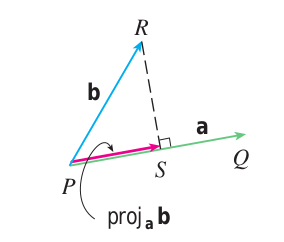
\includegraphics[scale=0.5]{proj}
%\end{defn}
\paragraph{Scalar Projection} \begin{defn}
	\textbf{Scalar Projection} of $\underline{v}$ onto $\underline{u}$ is given by: $comp_{\underline{u}}(\underline{v})=\frac{\underline{u}\cdot \underline{v}}{|\underline{u}|}$
\end{defn}
\paragraph{Vector Projection} \begin{defn}
	\textbf{Vector Projection} of $\underline{v}$ onto $\underline{u}$ is given by: $proj_{\underline{u}}(\underline{v})=\left(\frac{\underline{u}\cdot \underline{v}}{|\underline{u}|^2}\right)\underline{u}$
\end{defn}
\subsubsection{Cross Product} 
\begin{defn}
	Let $\underline{v}_1=\langle a_1, a_2, a_3 \rangle, \underline{v}_2=\langle b_1,b_2,b_3 \rangle.$ The \textbf{cross product} of $\underline{v}_1,\underline{v}_2$ is given by $\underline{v}_1 \times \underline{v}_2 = \langle a_2b_3-a_3b_2,a_3b_1-a_1b_3,a_1b_2-a_2b_1 \rangle$ 
\end{defn}
Can be obtained from the determinant of:
\begin{align*}
	\left[\begin{matrix}
	\underline{i} & \underline{j} & \underline{k}
	\\ a_1 & a_2 & a_3
	\\ b_1 & b_2 & b_3 
	\end{matrix}\right]
\end{align*}
\begin{thm}
	\begin{enumerate}[i)]
		\item $|\underline{v}_1 \times \underline{v}_2|=|\underline{v}_1||\underline{v}_2|\sin{\theta}, 0\leq \theta \leq \pi $
		\\ In fact, $|\underline{v}_1||\underline{v}_2|\sin{\theta}$ is the area of the parallelogram determined by $\underline{v}_1,\underline{v}_2$
		\item Two nonzero vectors $\underline{v}_1,\underline{v}_2$ are parallel if and only if $\underline{v}_1 \times \underline{v}_2=0$. 
	\end{enumerate}
\end{thm}
\subsection{Lines}
\paragraph{Equation of a Line}
\begin{defn}
	The equation of a line is given by: $\underline{r}=\underline{r}_0-t\underline{v}$.
	\\ Now let $\underline{r}=\langle x,y,z \rangle, \underline{r}_0=\langle x_0, y_0, z_0 \rangle, \underline{v}=\langle a,b,c \rangle$.
	\\ The \textbf{parametric equations} of the line L passing through $(x_0,y_0,z_0)$ and parallel to $\underline{v}=\langle a,b,c \rangle$ is given by: $x=x_0+at,y=y_0+bt,z=z_0+ct$
	\\ Solving for $t$ produces the \textbf{symmetric equations} of the line L: $\frac{x-x_0}{a}=\frac{y-y_0}{b}=\frac{z-z_0}{c}$
\end{defn}
\begin{defn}
	$2$ lines are \textbf{skew lines} if they are not parallel and do not intersect.
\end{defn}
\subsection{Planes}
What determines a plane in 3-D?
\begin{itemize}
	\item 3 noncolinear points in the plane.
	\item 2 nonparallel vectors and a point $p_0$ in the plane.
	\item a point $p_0$ in the plane and a vector $\underline{n}$ (\textbf{normal vector}) that is perpendicular to the plane. 
\end{itemize}
\begin{defn}
	Let $p_0=(x_0,y_0,z_0)$ and $p=(x,y,z)$.
	\\$\underline{n}\cdot (\underline{r}-\underline{r}_0)=0$ is the \textbf{vector equation} of the plane.
	\\$\underline{r}=\langle x,y,z \rangle, \underline{r}_0=\langle x_0,y_0,z_0 \rangle, \underline{n}=\langle a,b,c \rangle$  
	\\ $a(x-x_0)+b(y-y_0)+c(z-z_0)=0$ is the \textbf{scalar equation} of the plane that contains $p_0=(x_0,y_0,z_0)$ and is perpendicular to $\underline{n}$. 
	\\ $ax+by+cz+d=0$ is the \textbf{linear equation for the plane}.
\end{defn}
\begin{thm}
	$\underline{v}_1 \times \underline{v}_2$ is orthogonal to $\underline{v}_1$ and $\underline{v}_2$.
\end{thm}
\subsection{Right-Hand Rule} If the finger of your right hand curl in the direction of rotation from $\underline{a}$ to $\underline{b}$ through $\theta$ ($0^{\degree}\leq \theta \leq 180^{\degree})$, then your thumb points in the direction of $\underline{a} \times \underline{b}$.
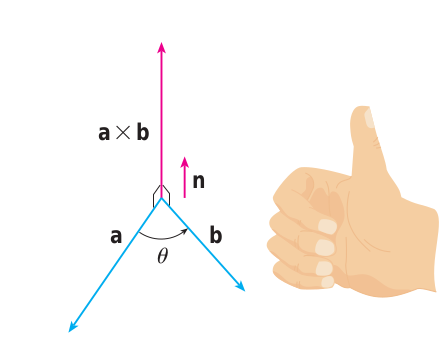
\includegraphics[scale=0.4]{rhr}
\subsection{Vector Functions and Space Curves}
\paragraph{Vector Functions}
\begin{defn}
	We say $\underline{r}(t)=\langle f(t),g(t),h(t) \rangle =f(t)\underline{i}+g(t)\underline{j}+h(t)\underline{k}$ is a \textbf{vector function}.
\end{defn}
\begin{defn}
	$f(t),g(t),h(t)$ are the \textbf{component functions} of $\underline{r}(t)$. The \textbf{domain} is the set $t\in \mathbb{R}$ s.t $f,g,h$ are defined at $t$.
\end{defn}
\begin{defn}
	The \textbf{limit} of $\underline{r}$ is defined by taking the limits of its component functions, that is: $$\lim_{t\to a}\underline{r}(t)=\langle \lim_{t\to a} f(t),\lim_{t\to a}g(t),\lim_{t\to a}h(t) \rangle$$
\end{defn}
\begin{defn}
	A vector function $\underline{r}$ is \textbf{continuous} at a if $$\lim_{t \to a}\underline{r}(t)=\underline{r}(a)$$
	\\$\underline{r}$ is \textbf{continuous} at a if and only if $f,g,h$ also are.
\end{defn}
\begin{defn}
	Let $f,g,h$ be continuous on an interval $I$. Let $C$ be the set of points $(x,y,z)$ satisfying 
	\begin{equation}
		x=f(t),y=g(t),z=h(t)
	\end{equation}
	for any $t$ in $I$. We say $C$ is a space curve and the equations given by equation (1) are its \textbf{parametric equations}.
	\\ We say $t$ is a \textbf{parameter}.
\end{defn}
\subsection{Arc Length, Curvature and the TNB Frame}
\begin{defn}
	The \textbf{derivative} of a vector function $\underline{r}(t)$ is given by: 
	\begin{equation*}
			\lim_{h\to 0}\frac{\underline{r}(t+h)-\underline{r}(t)}{h}=\underline{r}'(t)=\frac{d\underline{r}}{dt}
	\end{equation*}
 if it exists.
\end{defn}
\begin{thm}
	If $\underline{r}(t)=\langle f(t),g(t),h(t)\rangle$ and $f,g,h$ are differentiable, then $\underline{r}'(t)=\langle f'(t),g'(t),h'(t)\rangle$
\end{thm}
\begin{defn}
	We say $\underline{r}'(t)$ is the \textbf{tangent vector} of $\underline{r}(t)$ at $t$.
\end{defn}
\paragraph{Arc Length}
\begin{defn}
	Suppose we have a curve given by $\underline{r}(t)=\langle f(t),g(t),h(t)\rangle$ with $a\leq t \leq b$ and $f',g',h'$ are continuous. The \textbf{arc length} is defined as $$\int_{a}^{b}|\underline{r}'(t)| dt=\int_{a}^{b}\sqrt{\left(\frac{dx}{dt}\right)^2+\left(\frac{dy}{dt}\right)^2+\left(\frac{dz}{dt}\right)^2} dt$$
	\\ The \textbf{arc length function} is given by: $$s(t)=\int_{a}^{t}|\underline{r}'(u)|du$$
\end{defn}
\begin{defn}
	A \textbf{parametrization} of a curve $C$ is a representation of $C$ by a vector function using arc length.
\end{defn}
\paragraph{Curvature} \begin{defn}
A parametrization $\underline{r}(t)$ of $C$ is \textbf{smooth} on an interval $I$ if $\underline{r}'(t)$ is continuous and $\underline{r}'(t)\neq 0$ on $I$. A curve $C$ is \textbf{smooth} if it has a smooth parametrization. 
\end{defn}
\paragraph*{TNB Vectors}
\begin{defn}
	The \textbf{unit tangent vector} of $\underline{r}(t)$ is given by $$\underline{T}(t)=\frac{\underline{r}'(t)}{|\underline{r}'(t)|}$$
	The \textbf{unit normal vector} of $\underline{r}(t)$ is given by $$\underline{N}(t)=\frac{\underline{T}'(t)}{|\underline{T}'(t)|}$$
	The \textbf{binormal vector} of $\underline{r}(t)$ is given by $$\underline{B}(t)=\underline{T}(t)\times \underline{N}(t)$$
	They are all pairwise orthogonal and are of unit length.
\end{defn}
\begin{defn}
	The \textbf{curvature} $\kappa$ of $C$ is the length of the derivative of $\underline{T}(s)$, given by: $$\kappa =\left|\frac{dI}{dS}\right|$$
	$$\kappa (t)=\left|\frac{\underline{T}'(t)}{\underline{r}'(t)}\right|=\frac{|\underline{r}'(t)\times \underline{r}''(t)|}{|\underline{r}'(t)|^3}$$
\end{defn}
\subsection{Velocity \& Acceleration}
\begin{defn}
	Given a curve $C$ denoted by $\underline{r}(t)$, the \textbf{velocity} of $\underline{r}(t)$ is given by: $$\underline{r}'(t)=\lim_{h\to 0} \frac{\underline{r}(t+h)-\underline{r}(t)}{h}=\underline{v}(t)$$
\end{defn}
Note that speed is given by $|\underline{r}'(t)|=|\underline{v}(t)|$
\begin{defn}
	The \textbf{acceleration} of $\underline{r}(t)$ is $$\underline{a}(t)=\underline{r}''(t)=\underline{v}'(t)$$
\end{defn}
\paragraph{Components of Acceleration}~
\\ $\underline{a}(t)$ can be expressed purely in terms of $\underline{T}$ and $\underline{N}$ like so: $$\underline{a}=\underbrace{v'}_{a_T}\underline{T}+\underbrace{\kappa v^2}_{a_N} \underline{N}$$
One can also show: 
$$a_T=\frac{\underline{r}'(t)\cdot \underline{r}''(t)}{|\underline{r}'(t)|}$$
$$a_N=\frac{|\underline{r}'(t)\times r''(t)|}{|\underline{r}'(t)|}$$
\section{Multi-variable Functions}
\begin{defn}
	A \textbf{function of two variables} is a rule that assigns to each ordered pair of real numbers $(x,y)$ a real number $f(x,y)$ when $(x,y)$ is in the \textbf{domain} $D$ of $f$.
	\\\textbf{Domain} of $f$ is $D=\{(x,y):f(x,y)\text{ is defined}\}\subseteq\mathbb{R}^2$
	\\\textbf{Range} of $f$ is $\{f(x,y):(x,y)\in D\}\subseteq \mathbb{R}$
	\\\textbf{Graph} of $f$ is the set $\{(x,y,z)\in D \text{ and }z=f(x,y)\}\subseteq \mathbb{R}^3$
\end{defn}
\subsection{Contour Maps}
\begin{defn}
	We can represent functions $f(x,y)$ by taking horizontal slices of their graphs. These slices indicate height. The slices or \textbf{level curves} of $f(x,y)$ are the curves with equations $f(x,y)=k$ where $k$ is a constant in the range of $f$. If we draw the level curves we obtain a \textbf{contour map} of $f$.
\end{defn}
\subsection{Level Surfaces} To understand graphs of functions of $3$ variables, we draw \textbf{level surfaces}.
\subsection{Limits and Continuity}
\begin{defn}
	Let $f$ be a function of two variables whose domain $D$ includes points that are arbitrarily close to $(a,b)$. We say the \textbf{limit} of $f(x,y)$ as $(x,y)$ approaches $(a,b)$ is $L$: 
	$$\lim_{(x,y)\to (a,b)}f(x,y)=L$$
	if $\forall \varepsilon>0 \ \exists \delta>0$ s.t. if $(x,y)$ is in $D$ and $0<\sqrt{(x-a)^2+(y-b)^2}<\delta \implies |f(x,y)-L|<\varepsilon$
\end{defn}
\paragraph{Limit Laws}
\begin{thm}
	If the limits $\lim_{(x,y)\to(a,b)}f(x,y)$ and $lim_{(x,y)\to(a,b)}g(x,y)$ exist, then
	\begin{enumerate}[i)]
		\item $\lim_{(x,y)\to (a,b)}c (f(x,y))=c \lim_{(x,y)\to (a,b)}f(x,y)$
		\item $\lim_{(x,y)\to (a,b)}(f(x,y)+g(x,y))=\lim_{(x,y)\to (a,b)}f(x,y)+\lim_{(x,y)\to(a,b)}g(x,y)$
		\item $\lim_{(x,y)\to (a,b)}f(x,y)g(x,y)=(\lim_{(x,y)\to(a,b)}f(x,y))(\lim_{(x,y)\to(a,b)}g(x,y))$
		\item $\lim_{(x,y)\to(a,b)} \frac{f(x,y)}{g(x,y)}=\frac{\lim_{(x,y)\to(a,b)}f(x,y)}{\lim_{(x,y)\to(a,b)}g(x,y)}$, where denominator is nonzero.
	\end{enumerate}
\end{thm}
\paragraph{Continuity}
\begin{defn}
	A function $f$ is \textbf{continuous} at $(a,b)$ if $\lim_{(x,y)\to(a,b)}f(x,y)=f(a,b)$.
	\\ A function $f$ is \textbf{continuous} on a set $D$ if it is continuous at each $(a,b)$ in $D$.
\end{defn}
\begin{thm}
	$\frac{f}{g}$ is continuous if $f,g$ are continuous.
	\\ We can also show that polynomials and rational functions are continuous on their domains.
\end{thm}
\subsection{Partial Derivatives}
\begin{defn}
	The \textbf{partial derivative} of $f(x,y)$ with respect to $x$ is $$f(x,y)=\lim_{h\to 0}\frac{f(x+h,y)-f(x,y)}{h}$$
	In order to evaluate these limits, fix $y$ and differentiate wrt $x$ to obtain $f_x(x,y)$ or fix $x$ and wrt $y$ to get $f_y(x,y)$.
	\\ Notation: $$f_x=\frac{\partial f}{\partial x}=\frac{\partial z}{\partial x}=D_{x}f$$
	$$f_y=\frac{\partial f}{\partial y}=\frac{\partial z}{\partial y}=D_y f$$
\end{defn}
\paragraph{Higher Order Derivatives}
We can differentiate $f_x$ and $f_y$ to obtain
\begin{align*}
	&(f_x)_y=\frac{\partial}{\partial y}\left(\frac{\partial f}{\partial x}\right)=\frac{\partial^2 f}{\partial y \partial x}
	\\&(f_x)_x=\frac{\partial}{\partial x}\left(\frac{\partial f}{\partial x}\right)=\frac{\partial^2 f}{(\partial x)^2}
	\\&(f_y)_x=\frac{\partial}{\partial x}\left(\frac{\partial f}{\partial y}\right)=\frac{\partial^2 f}{\partial x \partial y}
	\\&(f_y)_y=\frac{\partial}{\partial y}\left(\frac{\partial f}{\partial y}\right)=\frac{\partial f^2}{(\partial y)^2}
\end{align*}
Note that, with $\partial$ notation, we derive from right to left, but with $f_x$ notation we derive from left to right.
\paragraph{Clairaut's Theorem:} 
\begin{thm}
	Suppose $f$ is defined on a disk $D$ that contains point $(a,b)$. If the functions $f_{xy},f_{yx}$ are continuous on $D$, then $f_{xy}(a,b)=f_{yx}(a,b)$
\end{thm}
\subsection{Tangent Planes} Let $f(x,y)$ be a function and let $S$ be the surface $z=f(x,y)$. 
\\ $T_1:$ tangent line in $x$-direction at $(x_0,y_0,f(x_0,y_0))$.
\\ $T_2:$ tangent line in $y$-direction at $(x_0,y_0,f(x_0,y_0))$.
\begin{defn}
	Define the \textbf{tangent plane} to $S$ at $(x_0,y_0,f(x_0,y_0))$ to be the plane that contains both $T_1,T_2$, given by: $$z=z_0+a(x-x_0)+b(y-y_0)$$
	\\ Its intersection with the plane $y=y_0$ (or $x=x_0$) is $T_1$ (or $T_2$)
	$$\implies T_1=z-z_0=a(x-x_0),T_2=z-z_0=b(y-y_0)$$
\end{defn}
\begin{thm}
	If $f$ has continuous partial derivatives, an equation of the tangent plane to $z=f(x,y)$ at $(x_0,y_0,f(x_0,y_0))$ is $$z-z_0=f_x(x_0,y_0)(x-x_0)+f_y(x_0,y_0)(y-y_0)$$
\end{thm}
\paragraph{Approximation Using Tangent Planes}
\begin{defn}
	The \textbf{linearization} of $f(x,y)$ at $(a,b)$ is defined as $$L(x,y)=f(a,b)+f_x(a,b)(x-a)+f_y(a,b)(y-b)$$
	The approximation $$f(x,y)\approx f(a,b)+f_x(a,b)(x-a)+f_y(a,b)(y-b)$$ is called the \textbf{linear approximation} or \textbf{tangent plane approximation} of $f$ at $(a,b)$.
\end{defn}
\begin{thm}
	If $f_x$,$f_y$ exist near $(a,b)$ and are continuous at $(a,b)$, then $f$ is differentiable at $(a,b)$.
\end{thm}
\section{How to Solve Problems}
\subsection{Series}
\paragraph{Representing a Function as a Power Series} Look for a familiar function that has a power series representation, plug it in and simplify. Integrate and differentiate as required.
\paragraph{Finding the Radius of Convergence} Usually involves the ratio test and checking when $r<1$.
\paragraph{Finding the Interval of Convergence} Use the radius of convergence and check if endpoints converge.
\paragraph{Finding the Sum of a Series} Look for a familiar series that can be represented as a function.
\paragraph{Using the Definition of Taylor Series} To find a power series representation or to find first few terms, just derive and use $c_n=\frac{f^{n}(a)}{n!}$.
\paragraph{Evaluating an Indefinite Integral with Series} Replace known function by a familiar series, try to cancel out other terms, integrate the series.
\paragraph{Evaluating a Limit with Series} Same as above for integrating.
\subsection{Vectors}
\paragraph{Compute Something} Compute what it asks for given the corresponding formula, whether it's the dot product, cross product, projection, etc.
\paragraph{Angle Between 2 Vectors} Use either the dot product or cross product.
\paragraph{Values for x Such that 2 Vectors are Orthogonal} Use the dot product and solve for it being $0$.
\paragraph{Finding a Parametric Equation of a Line} Use a point and a direction vector.
\paragraph{Finding the Equation of a Plane} Use a point and a normal vector.
\paragraph{Find Where a Line Intersects a Plane} Plug in parameters $(x,y,z)$ from line into the equation of a plane and solve for $t$ and get the corresponding point from the line with that value of $t$.
\paragraph{Distance from a Line to the Origin} Take $DV=\underline{a}$ and $\underline{b}$ some point on the line (usually $t=0$). Then $d=\frac{|\underline{a}\times \underline{b}|}{|\underline{a}|}$.
\paragraph{Are 2 Lines Skew, Parallel or Intersecting?} If $DV$ are multiples of each other, parallel. If you equate each component $x=x,y=y,z=z$ from both lines and you can solve the system, then they intersect. Otherwise, skew.
\paragraph{Angles Between Planes/Parallel or Perpendicular} To show parallel, compare $NV$. To show perpendicular, use the dot product. If neither, the angle can be computed with the dot product.
\paragraph{Line of Intersection of Two Planes} Find an intersecting point and use the cross product with both $NV$ to get a $DV$.  
\paragraph{Distance Between 2 Parallel Planes} Given plane equations of the form $ax+by+cz=d$, then distance $D=\frac{|d_1-d_2|}{\sqrt{a^2+b^2+c^2}}$
\paragraph{Distance Between a Point and a Plane} $p=(x_1,y_1,z_1)$, then $D=\frac{|ax_1+by_1+cz_1+d|}{\sqrt{a^2+b^2+c^2}}$
\paragraph{Diagonals of a Parallelogram} Given $\underline{u}$ and $\underline{v}$ that form the sides of a parallelogram, lengths of two diagonals are $|\underline{u}+\underline{v}|$ and $|\underline{u}-\underline{v}|$.
\subsection{Vector Functions}
\paragraph{Find the Domain of a Vector Function} Check where it isn't defined.
\paragraph{Limit of a Vector Function} Take the limit of each component.
\paragraph{Integral of a Vector Function} Take the integral of each component.
\paragraph{Curve of Intersection Between Cylinder and Plane} If you have a projection of a cylinder onto a circle like $x^2+y^2=16,z=0$, then you can write $x=4\cos t,y=4 \sin t, 0\leq t \leq 2\pi$. Take the plane, isolate for $z$ and plug in $x,y$ from circle. Then your vector function is given by $x \& y$ from circle and $z$ from plane with plugged in $x,y$.
\paragraph{Where does a Curve Intersect a Plane?}$xz$-plane $\implies y=0$, $xy$-plane $\implies z=0$, etc.
\paragraph{Parametric Equation of a Line at a Certain Point} Get $\underline{r}'(t)$ and plug in $t$ to get $DV$. Can use this $DV$ as a $NV$ for a normal plane to the curve.
\paragraph{Length of the Curve} Use arc length formula. 
\paragraph{Angle of Intersection of 2 Curves} Get the point where they intersect, then find tangents at those points and use dot product.
\paragraph{Reparametrizing a Curve} Given a point, get the corresponding $t$ value. Then measure arc length from $0$ to $t$ and solve for $t$ wrt $s$ and plug it into arc length formula wrt $t$, getting $r(t(s))$.
\paragraph{Computing $\underline{T}$ $\underline{N}$ $\underline{B}$, $\kappa$} Use the formulas.
\paragraph{Particle Velocity, Speed and Acceleration} Compute with formulas, note that speed is $|v(t)|$. Might have to work backwards by integrating if given acceleration and/or velocity to get position, don't forget constant.
\paragraph{Acceleration and Normal Components of Acceleration Vector} Formulas.
\subsection{Multi-variable Functions}
\paragraph{Showing Limits Don't Exist} Approach from different lines, show that they approach different values.
\paragraph{Where is a Function Continuous} Check if polynomial, rational function, composition of continuous functions and check domain.
\section{Problems}
\subsection{Important Problems}
\subsubsection{Assignment 1} 14, 15, 16, 17, 18, 19
\subsubsection{Assignment 2} 2, 3, 5, 7, 8, 9, 10, 11, 12, 14, 16, 17
\subsection{Review Problems}
\begin{itemize}
	\item p.811-812: 5-16, 35-44, 53-56, 61-65, 73-80
	\item p.882-883: 4-7, 9, 15-25, 27
	\item p.922: 2, 3, 5, 6, 8, 9, 10, 11, 12, 13, 17, 19, 22
	\item Section 14.2: 9, 11, 15, 21, 29-38
\end{itemize}
\section{Misc}
\begin{align}
	& \lim_{n\to \infty}arctan(n)=\frac{\pi}{2}
	\\&\frac{d}{dx}\left(a^x\right)=a^x log(a)
\end{align}
\end{document}